View demo code of this section: \democode{05}{5.1_Quantum_Neural_Network} \ \democodegithub{05}{5.1_Quantum_Neural_Network}
\subsubsection{Background}
In this subsection, we will go through how to create a quantum neural network to address the issue of iris classification in supervised learning, which is a challenge in classical machine learning.

The iris dataset is a popular dataset in classical machine learning. This dataset comprises 150 samples (split into three subgenus: setosa, versicolor, and virginica, with 50 samples each), and each sample has four features: sepal length, sepal width, petal length, and petal width.

We select the first 100 samples (setosa and versicolor), and 80 samples will be randomly chosen from them as the training set. After that, we built a quantum neural network to train the quantum classifier (ansatz). The remaining 20 samples are then sent to a classification test after learning, with the goal of achieving the greatest prediction accuracy possible.

First, we divide 100 samples into 80 training samples and 20 testing samples. Second, we calculate the parameters required to build an encoder based on the classical data of the training samples. Third, we create an encoder to encode the classical data of the training samples to the quantum state. Fourth, we design an ansatz and train its parameters with the proposed quantum neural network layer and MindSpore operators, which  will enable us to obtain the final classifier. Finally, we classify the remaining 20 testing samples and acquire the accuracy of the predictions.

\subsubsection{Data initialization}
In the first place, we should import the iris dataset.

\begin{lstlisting}
from sklearn import datasets

iris_dataset = datasets.load_iris()
\end{lstlisting}

Since we just need to select the first 100 samples, then execute the following command.

\begin{lstlisting}
import numpy as np

x = iris_dataset.data[:100, :].astype(np.float32)
x_feature_names = iris_dataset.feature_names
y = iris_dataset.target[:100].astype(int)
y_target_names = iris_dataset.target_names[:2]
\end{lstlisting}

In order to have a more intuitive understanding of the dataset consisting of these 100 samples, we could draw a scatterplot of the composition between the different features of all the samples by executing the following command.

\begin{lstlisting}
import matplotlib.pyplot as plt

feature_name = {0: 'sepal length', 1: 'sepal width', 2: 'petal length', 3: 'petal width'}
axes = plt.figure(figsize=(23, 23)).subplots(4, 4)

colormap = {0: 'r', 1: 'g'}
cvalue = [colormap[i] for i in y]

for i in range(4):
    for j in range(4):
        if i != j:
            ax = axes[i][j]
            ax.scatter(x[:, i], x[:, j], c=cvalue)
            ax.set_xlabel(feature_name[i], fontsize=22)
            ax.set_ylabel(feature_name[j], fontsize=22)

plt.show()
\end{lstlisting}

%\begin{figure*}[t]
%\centering
%\label{irisdatasetfigure}
%\includegraphics[width=0.8\textwidth]{5.1_figures/irisdataset_figure.eps}
%\caption{Visualization of iris dataset}
%\end{figure*}

%As seen in the images above, the red dots indicate samples with the label ``0", while the green dots represent samples with the label ``1".

\subsubsection{Encoder and Ansatz}
Following that, we compute the parameters required to build the encoder.  Activate the upcoming command.

\begin{lstlisting}
alpha = x[:, :3] * x[:, 1:]
x = np.append(x, alpha, axis=1)
\end{lstlisting}

Constructing features is a common technique in data preprocessing. Therefore, it can be found that each sample has 7 features at this time, the first four feature values are the original feature values, and the last three feature values are the ones calculated by the above preprocessing. The specific calculation formula is as follows:

\begin{eqnarray}\label{5.1dataprocessing}
    X_{i+4}^{j} = X_{i}^{j} * X_{i+1}^{j},
\end{eqnarray}
where $i = 0, 1, 2$ and $j = 1, 2, \cdots, 100$.

At last, we separate the current data set into a training set and a testing set by running the command below.

\begin{lstlisting}
from sklearn.model_selection import train_test_split

x_train, x_test, y_train, y_test = train_test_split(x, y, test_size=0.2, random_state=0, shuffle=True)
\end{lstlisting}

At this point there are 80 samples in the training set and 20 samples in the testing set, each with 7 features.

Next, we need to build an encoder in MindSpore Quantum to encode classical data into quantum states.

Here, the encoding method we employ is IQP encoding (Instantaneous Quantum Polynomial encoding). Generally speaking, the method of building the encoder is not set in stone, instead, many encoding techniques can be used depending on the demands of the issue at hand, and the encoder may occasionally be modified to improve performance.

The values of the parameters $\alpha_0$, $\alpha_1$, $\cdots$,$\alpha_6$ in the encoder are substituted with the 7 feature values obtained in the data processing of Eq.~\eqref{5.1dataprocessing}.

Now, we can build the quantum circuit of encoder in \MindQuantum\ (see Fig.~\ref{5.1encoder-circuit}) through the following code.

\begin{lstlisting}
from mindquantum import *

encoder = Circuit()

encoder += UN(H, 4)
for i in range(4):
    encoder += RZ(f'alpha{i}').on(i)
for j in range(3):
    encoder += X.on(j+1, j)
    encoder += RZ(f'alpha{j+4}').on(j+1)
    encoder += X.on(j+1, j)

encoder = encoder.no_grad()
encoder.svg()
\end{lstlisting}

\begin{figure}[H]
    \centering
    \includegraphics[width=0.49\textwidth]{5.1_figures/encoder-circuit.eps}
    \caption{IQP Encoder}
    \label{5.1encoder-circuit}
\end{figure}

As can be seen from the encoder circuit, the quantum circuit consists of 17 quantum gates, of which 7 are
parameterized quantum gates and the parameters are $\alpha_0$, $\alpha_1$, $\cdots$,$\alpha_6$, respectively. The number of qubits regulated by the encoder circuit is 4.

Furthermore, we need to build an ansatz in MindSpore Quantum.

Like the encoder, the building strategy used by ansatz is flexible, allowing us to examine the effectiveness of various strategies.

In this case, we apply \HardwareEfficientAnsatz. The encoding scheme is depicted in the following quantum circuit (see Fig.~\ref{5.1ansatz-circuit}) through the following code.

\begin{lstlisting}
ansatz = HardwareEfficientAnsatz(4, single_rot_gate_seq=[RY], entangle_gate=X, depth=3).circuit
ansatz.svg()
\end{lstlisting}

\begin{figure}[H]
    \centering
    \includegraphics[width=0.49\textwidth]{5.1_figures/ansatz-circuit.eps}
    \caption{Hardware Efficient Ansatz}
    \label{5.1ansatz-circuit}
\end{figure}

As can be seen from the ansatz circuit, the quantum circuit consists of 25 quantum gates, of which 16 are parameterized quantum gates and the parameters are $d0\_n0\_0$, $d0\_n1\_0$, $d0\_n2\_0$, $\cdots$,  respectively. The number of qubits regulated by the ansatz circuit is 4.

In such case, encoder and ansatz might create a whole quantum circuit (see Fig.~\ref{5.1total-circuit}) through the following code.

\begin{lstlisting}
circuit = encoder.as_encoder() + ansatz.as_ansatz()
circuit.svg()
\end{lstlisting}

\begin{figure}[H]
    \centering
    \includegraphics[width=0.49\textwidth]{5.1_figures/total-circuit.eps}
    \caption{The whole quantum circuit}
    \label{5.1total-circuit}
\end{figure}

\subsubsection{Hamiltonian}
We execute Pauli $Z$ operator measurement on the second and third qubits, respectively, to create the corresponding Hamiltonian. Execute the following code.

\begin{lstlisting}
hams = [Hamiltonian(QubitOperator(f'Z{i}')) for i in [2, 3]]
for h in hams:
    print(h)
\end{lstlisting}

\begin{lstlisting}
1 [Z2]
1 [Z3]
\end{lstlisting}

It can be seen from the above print that there are two Hamiltonians constructed at this time, which are to perform the Pauli $Z$ operator on the second and third qubits, respectively, and set the coefficients to 1. We will obtain two Hamiltonian measurement values by the Pauli $Z$ operator measurement.

If the first measurement value is larger, the sample will be classified into the class labeled ``0''.  Similarly, if the second measurement value is larger, this sample will be classified into the class with the label ``1''. By the training of the quantum neural network, it is expected that the first measurement value of the sample labeled ``0''  in the training sample is larger, and the second measurement value of the sample labeled ``1'' is larger. At last, this trained model is applied to predict the classification of new samples.

\subsubsection{Training}
We construct a quantum neural network by the following command.

\begin{lstlisting}
import mindspore as ms
from mindquantum.framework import MQLayer
from mindquantum.simulator import Simulator

ms.set_context(mode=ms.PYNATIVE_MODE, device_target="CPU")
ms.set_seed(1)
sim = Simulator('mqvector', circuit.n_qubits)
grad_ops = sim.get_expectation_with_grad(hams,
                                         circuit,
                                         parallel_worker=5)
QuantumNet = MQLayer(grad_ops)
QuantumNet
\end{lstlisting}

\begin{lstlisting}
MQLayer<
  (evolution): MQOps<4 qubits mqvector VQA Operator>
  >
\end{lstlisting}

As can be seen from the above print, we have successfully built a quantum machine learning layer, which can seamlessly form a larger machine learning network with other operators in MindSpore.

Next, we need to define the loss function and set the parameters to be optimized. After that, we will combine the built quantum machine learning layer and MindSpore operators to form a larger machine learning network. Finally, we will train the model. %Follow the command below.

\begin{lstlisting}
from mindspore import LossMonitor, Model
from mindspore.nn import SoftmaxCrossEntropyWithLogits, Adam, Accuracy
from mindspore.dataset import NumpySlicesDataset
from mindspore.train import Callback

loss = SoftmaxCrossEntropyWithLogits(sparse=True, reduction='mean')
opti = Adam(QuantumNet.trainable_params(), learning_rate=0.1)

model = Model(QuantumNet, loss, opti, metrics={'Acc': Accuracy()})

train_loader = NumpySlicesDataset({'features': x_train, 'labels': y_train}, shuffle=False).batch(5)
test_loader = NumpySlicesDataset({'features': x_test, 'labels': y_test}).batch(5)

class StepAcc(ms.Callback):
    def __init__(self, model, test_loader):
        self.model = model
        self.test_loader = test_loader
        self.acc = []

    def step_end(self, run_context):
        self.acc.append(self.model.eval(self.test_loader, dataset_sink_mode=False)['Acc'])

monitor = LossMonitor(16)

acc = StepAcc(model, test_loader)

model.train(20, train_loader, callbacks=[monitor, acc], dataset_sink_mode=False)
\end{lstlisting}

\begin{lstlisting}
epoch: 1 step: 16, loss is 0.6140301823616028
epoch: 2 step: 16, loss is 0.48262983560562134
epoch: 3 step: 16, loss is 0.43457236886024475
epoch: 4 step: 16, loss is 0.4101267457008362
epoch: 5 step: 16, loss is 0.4027639925479889
epoch: 6 step: 16, loss is 0.39859312772750854
epoch: 7 step: 16, loss is 0.39496558904647827
epoch: 8 step: 16, loss is 0.3970319926738739
epoch: 9 step: 16, loss is 0.3954522907733917
epoch: 10 step: 16, loss is 0.39520972967147827
epoch: 11 step: 16, loss is 0.3955090641975403
epoch: 12 step: 16, loss is 0.3953099250793457
epoch: 13 step: 16, loss is 0.39525243639945984
epoch: 14 step: 16, loss is 0.3952508568763733
epoch: 15 step: 16, loss is 0.39521533250808716
epoch: 16 step: 16, loss is 0.39519912004470825
epoch: 17 step: 16, loss is 0.39518338441848755
epoch: 18 step: 16, loss is 0.395169198513031
epoch: 19 step: 16, loss is 0.39515653252601624
epoch: 20 step: 16, loss is 0.3951443135738373
\end{lstlisting}

The loss value keeps dropping during training and tends to stable about 20 iterations before convergent at roughly 0.395.

Based on the above convergence situation, we may present the accuracy of the model's predictions during the training process. %Run the following code.

\begin{lstlisting}
plt.plot(acc.acc)
plt.title('Statistics of accuracy', fontsize=20)
plt.xlabel('Steps', fontsize=20)
plt.ylabel('Accuracy', fontsize=20)

plt.show()
\end{lstlisting}

\begin{figure}[H]
    \centering
    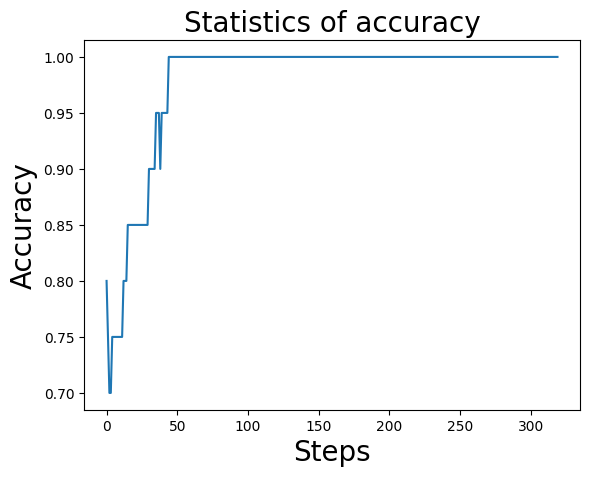
\includegraphics[width=0.4\textwidth]{5.1_figures/Statistics_of_accuracy.png}
    \caption{Statistics of accuracy}
    \label{5.1Statistics_of_accuracy}
\end{figure}

As can be seen from the Fig.~\ref{5.1Statistics_of_accuracy}, the prediction accuracy has converged to 1.00 after about 50 steps.

\subsubsection{Prediction}
Finally, we apply the trained model on the testing set.
\begin{lstlisting}
from mindspore import ops

predict = np.argmax(ops.Softmax()(model.predict(ms.Tensor(x_test))), axis=1)
correct = model.eval(test_loader, dataset_sink_mode=False)

print("Predicted classification result:", predict)
print("Actual classification result:", y_test)

print(correct)
\end{lstlisting}

\begin{lstlisting}
Predicted classification result: [0 1 0 1 1 1 0 1 1 1 1 1 1 0 0 0 0 0 0 0]
Actual classification result: [0 1 0 1 1 1 0 1 1 1 1 1 1 0 0 0 0 0 0 0]
{'Acc': 1.0}
\end{lstlisting}

As seen in the print above, the model's prediction accuracy has reached $100\%$, meaning that the anticipated classification results are perfectly consistent with the actual classification results.
